\section{Results and Discussion}
\label{sec:results}

This section evaluates unimodal and multimodal architectures on Emotion Detection, Irony Detection, and Semiotic Relation Detection. Rather than targeting state-of-the-art performance, we use these baselines to probe the corpus: we measure the contribution of visual features (text-only vs.\ Dual-Encoder), the informativeness of the auxiliary annotation layers (correlation prompting), and the behavior of Pixtral 12B, also disaggregated across semiotic subsets. Discriminative results are means over three training seeds; we describe an effect as consistent when it holds in all three seeds.

\subsection{Emotion Detection}
\label{sec:emotion_results}

Emotion detection represents the most challenging benchmark due to the high cardinality of the ten-class label space and the multi-label nature of affective expression in social media. Exploratory experiments attempting to collapse co-occurring emotions into single-label multiclass dyads under Plutchik's taxonomy or Ekman's basic emotions \cite{ekman1992argument} suffered from acute class sparsity and severe majority-class collapse. Recasting the task as a 10-dimensional multi-label binary problem over Plutchik's primary emotions (plus \textit{Love} and \textit{Neutral}) resolved this structural bottleneck.

Table~\ref{tab:emotion_baselines} summarizes the discriminative baselines. On the textual test set, the Step~1 encoder reaches a Macro $F_1$ of $0.506$. Further in-domain fine-tuning on raw text brings only a marginal change ($0.515$), whereas fine-tuning with correlation prompts raises performance to $0.530$, outperforming the raw Step~2 encoder in all three seeds.

On the multimodal test set, the text-only probe reaches $0.424$. Neither visual features ($0.432$) nor correlation prompts ($0.426$) improve it consistently on their own, but their combination yields $0.505$ ($+8.1$ points), exceeding both single-source configurations in every seed. Visual context and auxiliary annotations are therefore complementary for emotion: telling the classifier the target and figurative labels narrows down the ten emotions to a few likely candidates, allowing the visual features to separate categories with strong contextual ties such as \textit{Disgust} ($0.418 \rightarrow 0.589$) and \textit{Surprise} ($0.242 \rightarrow 0.379$). An inspection of the per-emotion confusion matrices confirms that this gain stems from genuine recovery of difficult affective instances rather than decision-threshold shifts: true positives increase from $7.0$ to $10.7$ for \textit{Disgust} (recall $37\% \rightarrow 56\%$) and from $3.7$ to $6.0$ for \textit{Surprise} (recall $23\% \rightarrow 38\%$), while false positive rates remain stable.

The ablation in Table~\ref{tab:emotion_baselines} shows the effect of also verbalizing the semiotic relation. On the textual test set, an encoder trained with the relation on its multimodal training rows improves to $0.544$, but on the multimodal test set the corresponding Dual-Encoder drops to $0.458$, below the configuration without the relation in all three seeds. Since the relation describes how text and image interact, it partly duplicates the information carried by the visual features rather than complementing it.

\begin{figure*}[!t]
\centering
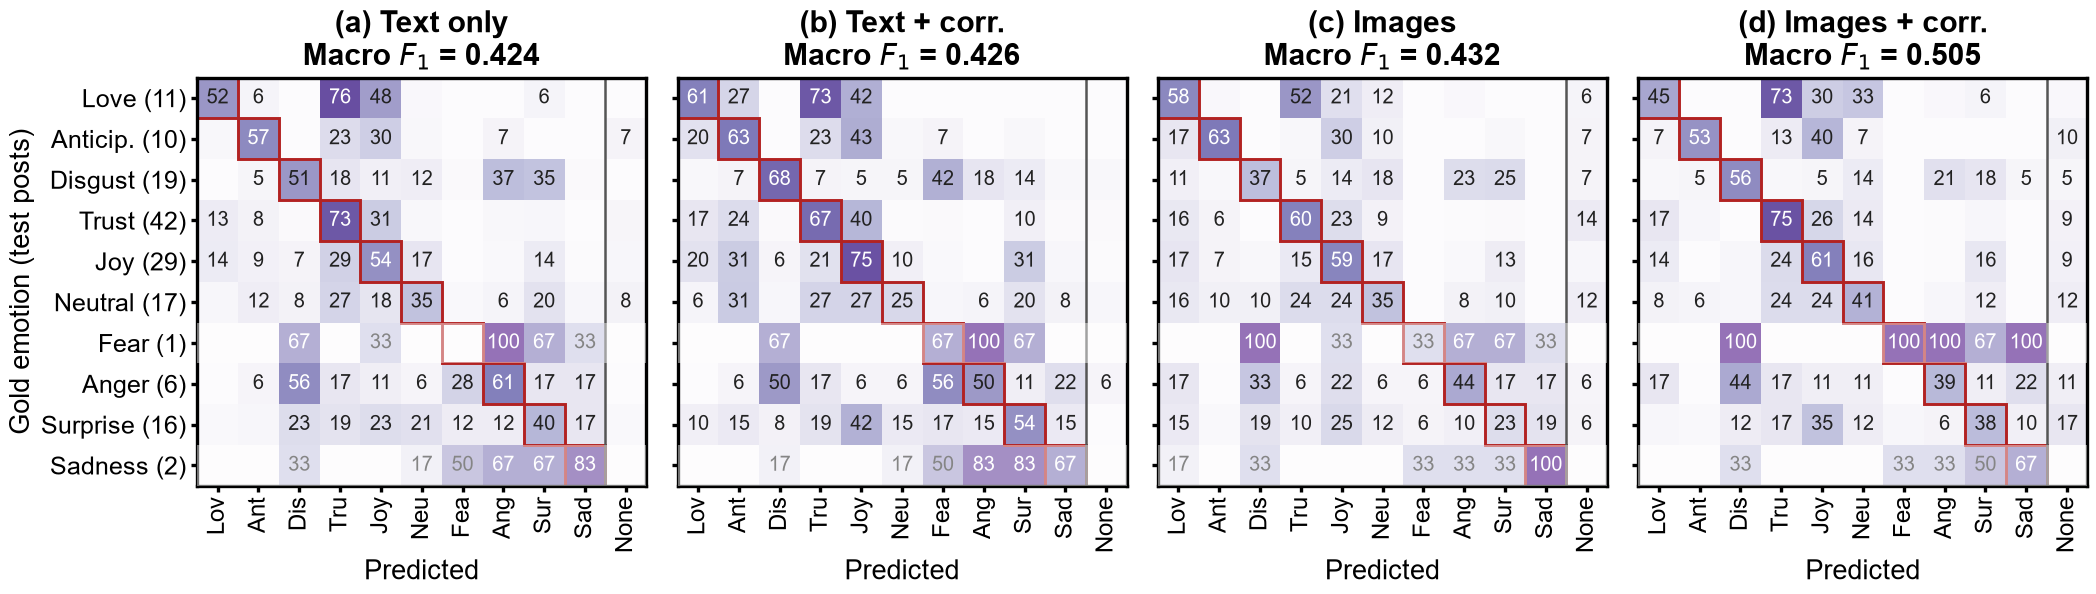
\includegraphics[width=\textwidth]{imgs/confusion_matrices_emotion.png}
\caption{Emotion detection on the multimodal test set ($N=129$), mean of three seeds. Each row is a gold emotion (number of test posts in brackets) and each cell is the percentage of those posts for which the column label was predicted; \textit{None} means that no label was predicted. Because a post can carry several emotions, rows can add up to more than 100\%. The red frame marks the correct label. \textit{Fear} and \textit{Sadness} have only 1 and 2 test posts and are shown faded.}
\label{fig:confusion_emotion}
\end{figure*}

Figure~\ref{fig:confusion_emotion} shows where these differences come from. Correlation prompts used on text alone add labels that the posts do not carry (Fig.~\ref{fig:confusion_emotion}b): the classifier predicts \textit{Fear} 14.3 times per run, against 3.3 without prompts and a single gold post, and 42\% of the \textit{Disgust} posts receive it. This raises the \textit{Disgust} recall from 51\% to 68\% but leaves the Macro $F_1$ unchanged. When images are added (Fig.~\ref{fig:confusion_emotion}d), \textit{Fear} falls back to 1.7 predictions and \textit{Disgust} is still recognized more often than without prompts (56\% against 37\% for the images alone), so the visual features appear to filter out part of what the prompt adds. Two groups of emotions remain confused in every setting: \textit{Love}, \textit{Trust}, and \textit{Joy} (\textit{Love} posts are labelled \textit{Trust} in 52\% to 76\% of the cases), and \textit{Disgust}, \textit{Anger}, and \textit{Surprise} (37\% and 35\% of \textit{Disgust} posts are labelled \textit{Anger} and \textit{Surprise} by the text-only model, 21\% and 18\% with images and prompts). Finally, the larger classes attract predictions: \textit{Trust} and \textit{Joy} are predicted 52.7 and 34.7 times by the text-only model, against 42 and 29 gold posts.

\begin{table}[!t]
\centering
\caption{Discriminative Baseline Performance in Emotion Detection (Mean of Three Seeds)}
\label{tab:emotion_baselines}
\footnotesize
\renewcommand{\arraystretch}{1.05}
\begin{tabular}{l c c}
\hline
\textbf{Configuration} & \textbf{Macro $F_1$} & \textbf{Micro $F_1$} \\
\hline
\multicolumn{3}{l}{\textit{Textual Test Set}} \\
Step 1 (EMiT + MultiEMiT) & 0.506 & 0.529 \\
Step 2 without correlations & 0.515 & 0.528 \\
Step 2 with correlations & \textbf{0.530} & \textbf{0.555} \\
\hline
\multicolumn{3}{l}{\textit{Multimodal Test Set}} \\
Text only & 0.424 & 0.492 \\
Text only with correlations & 0.426 & 0.499 \\
With images & 0.432 & 0.475 \\
With images and correlations & \textbf{0.505} & \textbf{0.529} \\
\hline
\multicolumn{3}{l}{\textit{Ablation: Relation Added to the Prompt}} \\
Step 2 with correlations (textual)$^{*}$ & 0.544 & 0.557 \\
Text only with correlations + relation & 0.439 & 0.515 \\
With images, correlations + relation & 0.458 & 0.520 \\
\hline
\multicolumn{3}{p{0.92\columnwidth}}{\footnotesize $^{*}$Relation verbalized on multimodal training rows only; textual test posts have no relation annotation.} \\
\end{tabular}
\end{table}

Turning to generative models (Table~\ref{tab:emotion_pixtral}), we selected the \textit{short} and \textit{long\_v1} templates for LoRA fine-tuning, as \textit{long\_v1} achieved the highest mean Macro $F_1$ across both decoding temperatures among the long zero-shot prompts. Fine-tuned Pixtral 12B (\textit{long\_v1}, $n=2$, $0.426$ at $T=0.1$) performs on par with the Dual-Encoder without correlations ($0.432$), but remains clearly below the correlation-prompted Dual-Encoder ($0.505$). The gap persists when the Dual-Encoder receives the same annotation layers as Pixtral, including the relation ($0.458$).

\begin{table}[!t]
\centering
\caption{Pixtral 12B versus Dual-Encoder in Emotion Detection ($T=0.1$ and $T=0.9$)}
\label{tab:emotion_pixtral}
\footnotesize
\renewcommand{\arraystretch}{0.92}
\begin{tabular}{l l c c}
\hline
\textbf{Model} & \textbf{Configuration} & \textbf{$T = 0.1$ $F_1$} & \textbf{$T = 0.9$ $F_1$} \\
\hline
\multicolumn{4}{l}{\textit{Discriminative Multimodal (Dual-Encoder)}} \\
BERT-ViT & FT (No Corr.) & 0.432 & 0.432 \\
BERT-ViT & FT (Corr.) & \textbf{0.505} & \textbf{0.505} \\
BERT-ViT & FT (Corr. + Rel.)$^{\dagger}$ & 0.458 & 0.458 \\
\hline
\multicolumn{4}{l}{\textit{Generative (Pixtral 12B)}} \\
Pixtral (long\_v1) & FT ($n=2$) & \textbf{0.426} & 0.359 \\
Pixtral (short) & FT ($n=2$) & 0.397 & \textbf{0.373} \\
Pixtral (short) & FT (all predictions) & 0.318 & 0.312 \\
Pixtral (short) & ZS (With Corr.) & 0.291 & 0.251 \\
Pixtral (long\_v1) & ZS (With Corr.) & 0.275 & 0.266 \\
Pixtral (medium) & ZS (With Corr.) & 0.269 & 0.262 \\
Pixtral (long\_v2) & ZS (No Corr.) & 0.266 & 0.237 \\
Pixtral (long\_v1) & ZS (No Corr.) & 0.261 & 0.261 \\
Pixtral (short) & ZS (No Corr.) & 0.261 & 0.291 \\
Pixtral (long\_v3) & ZS (With Corr.) & 0.258 & 0.262 \\
Pixtral (medium) & ZS (No Corr.) & 0.254 & 0.250 \\
Pixtral (long\_v2) & ZS (With Corr.) & 0.253 & 0.286 \\
Pixtral (long\_v1) & FT (all predictions) & 0.238 & 0.290 \\
Pixtral (long\_v3) & ZS (No Corr.) & 0.220 & 0.215 \\
\hline
\multicolumn{4}{p{0.95\columnwidth}}{\footnotesize Macro $F_1$. Dual-Encoder values are means over three training seeds and do not depend on decoding temperature; Pixtral values are means over three generation runs. Correlation-prompted Pixtral receives the per-instance annotations of the other layers (including the semiotic relation) and corpus-level correlation rules in the instruction. $^{\dagger}$Dual-Encoder input matched to Pixtral (relation included).} \\
\end{tabular}
\end{table}

\begin{table}[!t]
\centering
\caption{Impact of Truncation Parameter ($n$) on Pixtral Emotion Detection Performance}
\label{table:truncation_parameter}
\footnotesize
\begin{tabular}{c c}
\hline
\textbf{Number of Predictions ($n$)} & \textbf{Mean Macro $F_1$} \\
\hline
1 & 0.338 \\
2 & \textbf{0.389} \\
3 & 0.339 \\
4 & 0.325 \\
5 & 0.308 \\
\hline
\end{tabular}
\end{table}

After fine-tuning on emotion detection, Pixtral often failed to stop generating and instead returned long or repetitive lists of emotions (for example, listing four or five emotions in a row, or repeating the same pair of emotions). Because we used regular expressions to match all valid emotion names in the output, these extra guesses produced many false positives and caused a clear drop in performance (shown in the \textit{all predictions} rows of Table~\ref{tab:emotion_pixtral}). When comparing these raw outputs against the gold standard, we noticed that the model generally listed the most likely emotions first. We therefore tested truncating the extracted list to the first $n$ distinct emotions ($n = 1, \dots, 5$). As shown in Table~\ref{table:truncation_parameter} (averaged across the fine-tuned \textit{short} and \textit{long\_v1} prompts over both temperatures), performance peaks at $n=2$ (Mean Macro $F_1 = 0.389$), which also matches the maximum of two emotions requested in the prompt and the typical number of emotions per post in the dataset.

Disaggregating performance across semiotic subsets (Table~\ref{tab:semiotic_subsets_all}) reveals a divergence between discriminative and generative paradigms.

\begin{table}[!t]
\centering
\caption{Performance across Semiotic Subsets (Additive, Parallel, Divergent) for All Three Tasks}
\label{tab:semiotic_subsets_all}
\footnotesize
\renewcommand{\arraystretch}{1.02}
\begin{tabular}{l c c c}
\hline
\textbf{Task \& Model Setting} & \textbf{ADD} & \textbf{PAR} & \textbf{DIV} \\
\hline
\multicolumn{4}{l}{\textit{Emotion Detection (Micro $F_1$-score)}} \\
Dual-Encoder (No corr.) & 0.56 & 0.52 & 0.30 \\
Dual-Encoder (With corr.) & \textbf{0.58} & \textbf{0.55} & 0.42 \\
Dual-Encoder (Corr. + relation)$^{\dagger}$ & 0.55 & 0.51 & \textbf{0.47} \\
Pixtral 12B Zero-Shot (No corr.) & 0.29 & 0.23 & 0.44 \\
Pixtral 12B Zero-Shot (With corr.) & 0.32 & 0.30 & 0.43 \\
Pixtral 12B Fine-tuned ($n=2$, No corr.) & 0.33 & 0.41 & 0.41 \\
\hline
\multicolumn{4}{l}{\textit{Irony Detection (Micro $F_1$-score / Accuracy)}} \\
Dual-Encoder (No corr.) & \textbf{0.88} & 0.90 & \textbf{0.63} \\
Dual-Encoder (With corr.) & 0.84 & 0.90 & 0.53 \\
Dual-Encoder (Corr. + relation)$^{\dagger}$ & \textbf{0.88} & 0.93 & 0.54 \\
Pixtral 12B Zero-Shot (No corr.) & 0.14 & 0.00 & 0.18 \\
Pixtral 12B Zero-Shot (With corr.) & 0.57 & 0.78 & 0.57 \\
Pixtral 12B Fine-tuned (No corr.) & 0.87 & \textbf{1.00} & 0.58 \\
\hline
\multicolumn{4}{l}{\textit{Semiotic Relation Detection (Per-Class $F_1$-score, Pixtral long\_v1)}} \\
Text-only Probe (No corr.) & 0.69 & 0.46 & 0.56 \\
Dual-Encoder (No corr.) & 0.67 & 0.43 & 0.56 \\
Text-only Probe (With corr.) & 0.68 & \textbf{0.57} & 0.56 \\
Dual-Encoder (With corr.) & \textbf{0.71} & 0.48 & 0.56 \\
Pixtral 12B Zero-Shot (No corr.) & 0.62 & 0.00 & 0.56 \\
Pixtral 12B Zero-Shot (With corr.) & 0.61 & 0.00 & 0.56 \\
Pixtral 12B Three-Shot (With corr.) & 0.60 & 0.17 & \textbf{0.64} \\
Pixtral 12B Fine-tuned (No corr.) & \textbf{0.71} & 0.28 & 0.60 \\
\hline
\multicolumn{4}{p{0.88\columnwidth}}{\footnotesize $^{\dagger}$Ablation; input matched to Pixtral.} \\
\end{tabular}
\end{table}

The \textbf{Dual-Encoder} performs best on the \textit{Additive} and \textit{Parallel} subsets and worst on the \textit{Divergent} one ($0.30$ without correlations). Redundant or complementary text--image content reinforces the concatenated signal, whereas the tension between modalities in Divergent posts is hard to resolve for a linear classifier over frozen features. Correlation prompting brings its largest gain precisely on Divergent posts ($0.30 \rightarrow 0.42$), where auxiliary annotations such as irony help disambiguate the intended affect; this is also the only subset where adding the relation helps further ($0.47$).

\textbf{Zero-shot Pixtral 12B} shows the inverse pattern, performing best on \textit{Divergent} ($0.44$) and worst on \textit{Parallel} posts ($0.23$). Divergent commentary mostly consists of reaction memes and satire dominated by salient states (\textit{Joy}, \textit{Surprise}, \textit{Disgust}), which internet-scale pre-training may allow Pixtral to decode without task-specific training: it surpasses the unprompted Dual-Encoder on this subset ($0.44$ vs.\ $0.30$) and the correlation-prompted one ($0.42$). On literal Parallel posts, zero-shot Pixtral lacks domain priors and recovers only after fine-tuning ($0.41$).

\subsection{Irony Detection}
\label{sec:irony_results}

Irony relies on pragmatic incongruity, which may arise within the text itself or between text and image \cite{schifanella2016multimodal, cai2019multimodal}. Irony encoders are initialized from UmBERTo and trained with the same two-step procedure, using IronITA \cite{ironita2018} in the warm-up step and evaluating exclusively on held-out MultiEMiT instances (Table~\ref{tab:irony_baselines}).

On the textual test set, in-domain fine-tuning is the main driver: Step~2 raises Macro $F_1$ from $0.449$ to $0.506$ in all three seeds. Correlation prompts bring a further gain to $0.533$, improving the \textit{Sarcasm} class ($F_1$ from $0.27$ to $0.31$, with only 8 sarcastic test posts) and making training markedly more stable across seeds.

\begin{figure*}[!t]
\centering
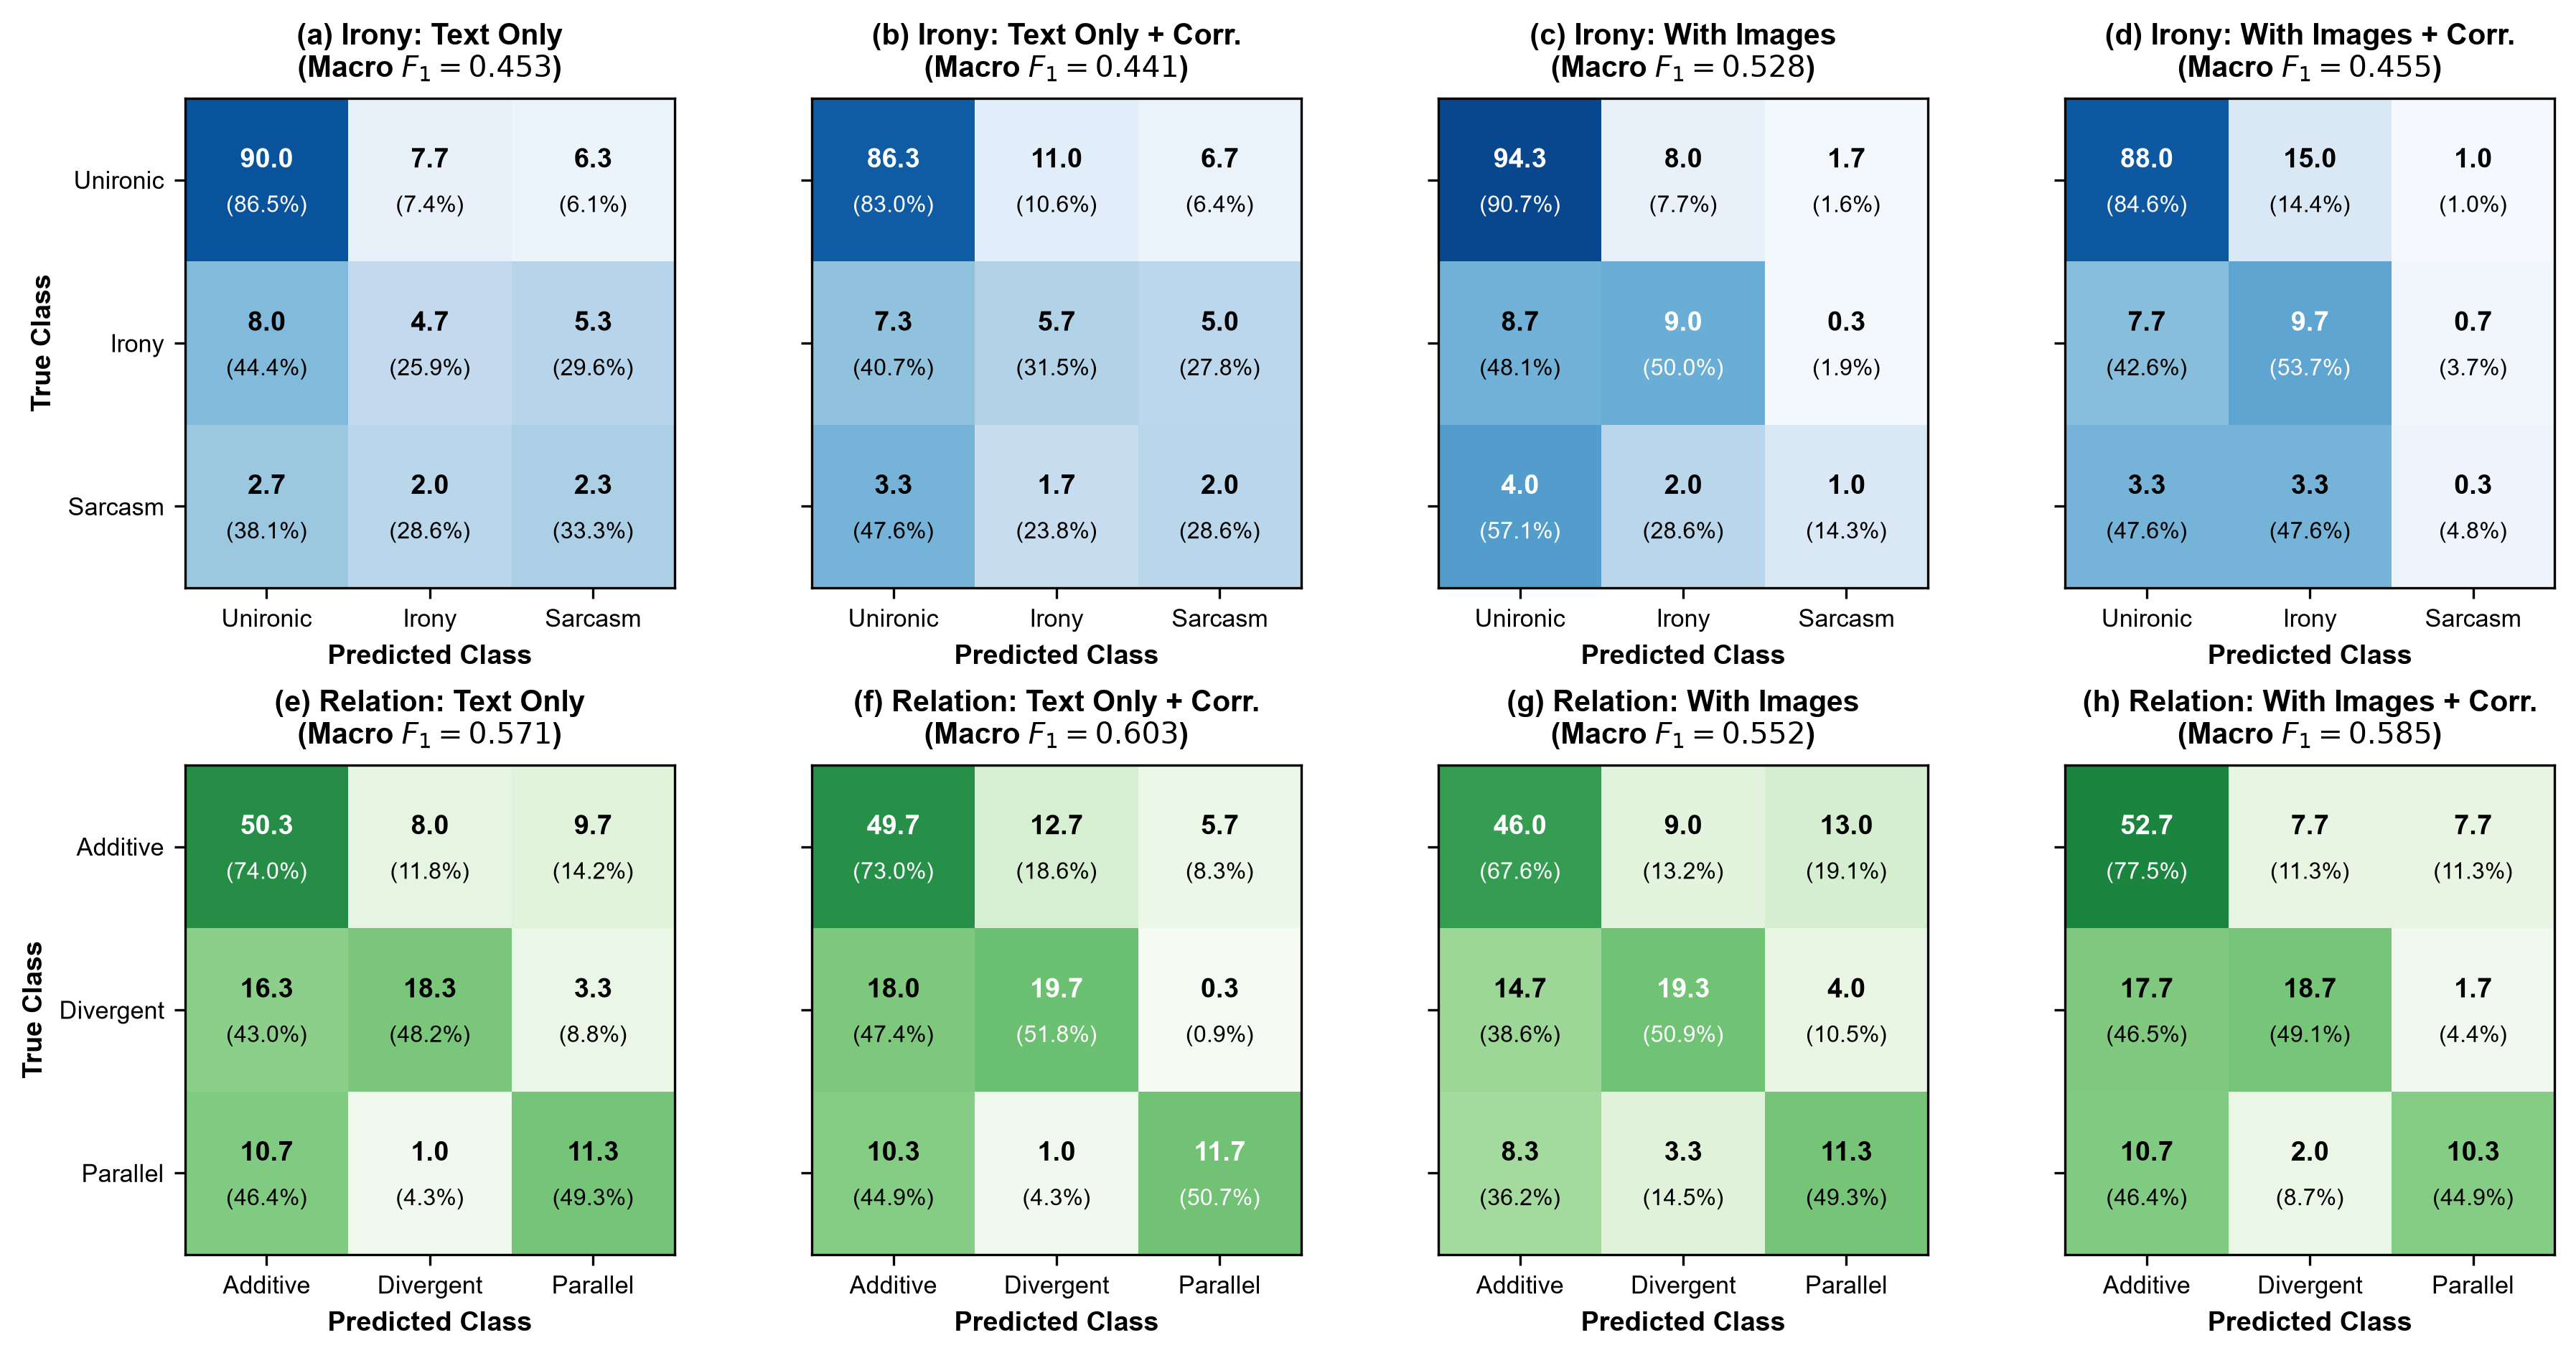
\includegraphics[width=0.98\textwidth]{imgs/confusion_matrices_irony_relation.png}
\caption{Three-seed averaged confusion matrices on the multimodal test set ($N=129$) for Irony Detection (top row, panels a--d) and Semiotic Relation Detection (bottom row, panels e--h), covering the complete $2\times2$ factorial design across input modalities (text only vs.\ with images) and correlation prompting. Each cell reports the mean number of test instances alongside the row-normalized percentage (true class recall). Cell shading reflects recall intensity.}
\label{fig:confusion_matrices}
\end{figure*}

On the multimodal test set, visual features provide the most robust effect observed in our study: the Dual-Encoder improves over the text-only probe from $0.453$ to $0.528$ ($+7.5$ points) in every seed, mainly by recognizing ironic posts (\textit{Irony} $F_1$ from $0.27$ to $0.49$). (For reference against severe class imbalance, a trivial majority-class baseline predicting \textit{Unironic} for all instances achieves an accuracy of $0.806$ but a Macro $F_1$ of only $0.298$, since minority figurative classes receive zero). This is consistent with the strong association between irony and Divergent text--image relations ($r = 0.407$, Section~\ref{sec:dataset_analysis}): part of the incongruity that defines multimodal irony is only observable in the image. Correlation prompts, by contrast, do not help on multimodal posts ($0.441$ text only, $0.455$ with images), and largely cancel the visual gain. Although the textual and multimodal correlation matrices share the same positive and negative signs, the target distribution shifts between partitions: in the textual dataset (which makes up 75.8\% of Step~2 training), \textit{Container} is a minority class (38.7\%) and 83.7\% of \textit{Container} posts are \textit{Unironic}, whereas in the multimodal dataset \textit{Container} becomes the majority (61.2\%) because viewers attach broadcast screenshots, and 27.8\% of ironic test posts (and 57.1\% of sarcastic test posts) target the \textit{Container}. When the prompt explicitly states that a post targets the \textit{Container}, the text encoder relies on the textual prior and pushes predictions toward \textit{Unironic}, overriding the visual contrast. Adding the relation to the prompt lowers performance further ($0.432$) and suppresses \textit{Sarcasm} entirely ($F_1 = 0$ in every seed): in the multimodal training split, \textit{Divergent} posts co-occur with \textit{Irony} 55 times versus \textit{Sarcasm} only 7 times, causing the linear classifier to favor \textit{Irony} whenever the relation is provided. With 25 ironic or sarcastic posts in the multimodal test set, these differences should be interpreted with caution.

An inspection of the confusion matrices (Fig.~\ref{fig:confusion_matrices}, top row) clarifies the exact error dynamics driving these shifts across the four factorial conditions. In the text-only probe (Fig.~\ref{fig:confusion_matrices}a), true ironic posts are correctly detected only 25.9\% of the time (4.7 out of 18 posts) and are frequently confused with sarcasm (29.6\%, 5.3 posts). Adding correlation prompts to text alone (Fig.~\ref{fig:confusion_matrices}b) yields only modest recall gains for irony (31.5\%, 5.7 posts) while increasing false alarms on sincere posts (from 7.4\% to 10.6\%, 11.0 posts). Incorporating visual representations in the Dual-Encoder without prompts (Fig.~\ref{fig:confusion_matrices}c) produces the sharpest behavioral improvement: true irony recall doubles to 50.0\% (9.0 posts) and confusion with sarcasm is virtually eliminated (dropping from 29.6\% to 1.9\%, 0.3 posts), while false sarcastic alarms on sincere instances drop to 1.6\%. When correlation prompts are combined with images (Fig.~\ref{fig:confusion_matrices}d), the model over-triggers irony on sincere posts: unironic false alarms jump to 14.4\% (15.0 posts), explaining the drop in precision and overall Macro $F_1$.

\begin{table}[!t]
\centering
\caption{Discriminative Baseline Performance in Irony Detection (Mean of Three Seeds)}
\label{tab:irony_baselines}
\footnotesize
\renewcommand{\arraystretch}{1.05}
\begin{tabular}{l c c}
\hline
\textbf{Configuration} & \textbf{Macro $F_1$} & \textbf{Micro $F_1$} \\
\hline
\multicolumn{3}{l}{\textit{Textual Test Set}} \\
Step 1 (IronITA + MultiEMiT) & 0.449 & 0.737 \\
Step 2 without correlations & 0.506 & 0.760 \\
Step 2 with correlations & \textbf{0.533} & \textbf{0.765} \\
\hline
\multicolumn{3}{l}{\textit{Multimodal Test Set}} \\
Text only & 0.453 & 0.752 \\
Text only with correlations & 0.441 & 0.729 \\
With images & \textbf{0.528} & \textbf{0.809} \\
With images and correlations & 0.455 & 0.760 \\
\hline
\multicolumn{3}{l}{\textit{Ablation: Relation Added to the Prompt}} \\
Step 2 with correlations (textual)$^{*}$ & 0.510 & 0.760 \\
Text only with correlations + relation & 0.425 & 0.760 \\
With images, correlations + relation & 0.432 & 0.786 \\
\hline
\multicolumn{3}{p{0.92\columnwidth}}{\footnotesize $^{*}$Relation verbalized on multimodal training rows only; textual test posts have no relation annotation.} \\
\end{tabular}
\end{table}

In the generative regime (Table~\ref{tab:irony_pixtral}), unprompted zero-shot Pixtral 12B collapses on figurative language (Macro $F_1 \leq 0.218$). Correlation prompts trigger the largest prompt effect observed in our study, raising zero-shot performance to $0.512$ with \textit{long\_v2} at $T=0.1$, close to the best Dual-Encoder ($0.528$), while LoRA fine-tuning reaches $0.454$ (\textit{long\_v2}, $T=0.9$). When the Dual-Encoder receives the same annotation layers as Pixtral ($0.432$), prompted Pixtral outperforms it, suggesting that a generative model can exploit explicit correlation rules more effectively than a linear probe exploits oracle labels on this sparse task.

\begin{table}[!t]
\centering
\caption{Pixtral 12B versus Dual-Encoder in Irony Detection ($T=0.1$ and $T=0.9$)}
\label{tab:irony_pixtral}
\footnotesize
\renewcommand{\arraystretch}{0.92}
\begin{tabular}{l l c c}
\hline
\textbf{Model} & \textbf{Configuration} & \textbf{$T = 0.1$ $F_1$} & \textbf{$T = 0.9$ $F_1$} \\
\hline
\multicolumn{4}{l}{\textit{Discriminative Multimodal (Dual-Encoder)}} \\
BERT-ViT & FT (No Corr.) & \textbf{0.528} & \textbf{0.528} \\
BERT-ViT & FT (Corr.) & 0.455 & 0.455 \\
BERT-ViT & FT (Corr. + Rel.)$^{\dagger}$ & 0.432 & 0.432 \\
\hline
\multicolumn{4}{l}{\textit{Generative (Pixtral 12B)}} \\
Pixtral (long\_v2) & ZS (With Corr.) & \textbf{0.512} & 0.396 \\
Pixtral (long\_v2) & FT (all predictions) & 0.405 & \textbf{0.454} \\
Pixtral (short) & ZS (With Corr.) & 0.348 & 0.298 \\
Pixtral (long\_v3) & ZS (With Corr.) & 0.340 & 0.281 \\
Pixtral (short) & FT (all predictions) & 0.329 & 0.394 \\
Pixtral (medium) & ZS (With Corr.) & 0.264 & 0.270 \\
Pixtral (long\_v1) & ZS (With Corr.) & 0.248 & 0.295 \\
Pixtral (long\_v2) & ZS (No Corr.) & 0.165 & 0.218 \\
Pixtral (long\_v3) & ZS (No Corr.) & 0.148 & 0.198 \\
Pixtral (long\_v1) & ZS (No Corr.) & 0.126 & 0.158 \\
Pixtral (short) & ZS (No Corr.) & 0.054 & 0.108 \\
Pixtral (medium) & ZS (No Corr.) & 0.051 & 0.137 \\
\hline
\multicolumn{4}{p{0.95\columnwidth}}{\footnotesize Macro $F_1$. Dual-Encoder values are means over three training seeds and do not depend on decoding temperature; Pixtral values are means over three generation runs. Correlation-prompted Pixtral receives the per-instance annotations of the other layers (including the semiotic relation) and corpus-level correlation rules in the instruction. $^{\dagger}$Dual-Encoder input matched to Pixtral (relation included).} \\
\end{tabular}
\end{table}

Examining irony across semiotic subsets (Table~\ref{tab:semiotic_subsets_all}) shows how models handle multimodal dissonance. All 23 \textit{Parallel} test posts are \textit{Unironic}. Fine-tuned Pixtral classifies all of them correctly ($1.00$), the Dual-Encoder produces occasional false positives ($0.90$--$0.93$), and unprompted zero-shot Pixtral hallucinates irony on every post. The \textit{Divergent} subset, where irony concentrates, remains the most challenging: the Dual-Encoder without correlations performs best ($0.63$), while all correlation-prompted configurations and fine-tuned Pixtral cluster between $0.53$ and $0.58$. On the \textit{Additive} subset, the discriminative models and fine-tuned Pixtral reach similar scores ($0.84$--$0.88$).

\FloatBarrier
\subsection{Semiotic Relation Detection}
\label{sec:relation_results}

Semiotic relation detection requires the model to categorize the interaction between modalities as Additive, Parallel, or Divergent. Because relation annotations exist only for posts with paired media, training and evaluation were restricted to the multimodal partition.

Table~\ref{tab:relation_baselines} summarizes the discriminative baselines. The fine-tuned UmBERTo classification head, reported as a reference, reaches the highest Micro $F_1$ ($0.66$) but a low Macro $F_1$ ($0.54$), as it frequently neglects the minority \textit{Parallel} class. (For reference against the 52.7\% majority class, a naive baseline predicting the dominant \textit{Additive} category yields Micro $F_1 = 0.527$ and Macro $F_1 = 0.230$). A linear classifier with balanced class weights on the same frozen text features yields a more balanced $0.571$, showing that the text alone carries partial cues about its relation to the image (e.g., purely descriptive commentary tends to accompany Parallel imagery). Correlation prompts raise this probe to $0.603$, the best Macro $F_1$ among discriminative configurations. With unscaled feature concatenation, adding visual features does not improve the text-only probe ($0.552$ without and $0.585$ with correlations); within the Dual-Encoder, however, correlation prompts help in every seed. The affective and figurative annotation layers, in particular irony, thus encode a substantial part of the cross-modal relation.

The semiotic relation confusion matrices (Fig.~\ref{fig:confusion_matrices}, bottom row) highlight the structural pull exerted by the dominant \textit{Additive} class (52.7\% of multimodal instances). In the text-only probe (Fig.~\ref{fig:confusion_matrices}e), 43.0\% of \textit{Divergent} posts (16.3 out of 38) and 46.4\% of \textit{Parallel} posts (10.7 out of 23) are misclassified as \textit{Additive}. Fusing visual features in the Dual-Encoder (Fig.~\ref{fig:confusion_matrices}g) reduces this majority-class pull: misclassifications into \textit{Additive} drop to 36.2\% for \textit{Parallel} (8.3 posts) and 38.6\% for \textit{Divergent} (14.7 posts), confirming that visual embeddings help separate literal accompaniment from affective contrast. When correlation prompts are supplied (Fig.~\ref{fig:confusion_matrices}h), the model sharpens its \textit{Additive} predictions (77.5\% recall), although \textit{Divergent} instances remain divided between correct predictions (49.1\%) and \textit{Additive} false negatives (46.5\%).

\begin{table}[!t]
\centering
\caption{Discriminative Baseline Performance in Semiotic Relation Detection (Mean of Three Seeds)}
\label{tab:relation_baselines}
\footnotesize
\renewcommand{\arraystretch}{1.05}
\begin{tabular}{l c c}
\hline
\textbf{Configuration} & \textbf{Macro $F_1$} & \textbf{Micro $F_1$} \\
\hline
\multicolumn{3}{l}{\textit{Fine-tuned UmBERTo Head (Reference)}} \\
Without correlations & 0.541 & 0.662 \\
With correlations & 0.542 & \textbf{0.664} \\
\hline
\multicolumn{3}{l}{\textit{Linear Classifier on Frozen Features}} \\
Text only & 0.571 & 0.620 \\
Text only with correlations & \textbf{0.603} & 0.628 \\
With images & 0.552 & 0.594 \\
With images and correlations & 0.585 & 0.633 \\
\hline
\end{tabular}
\end{table}

As detailed in Table~\ref{tab:relation_pixtral}, fine-tuned Pixtral 12B (\textit{long\_v1}, $0.613$ at $T=0.1$) is the best multimodal model for this task, outperforming the Dual-Encoder with ($0.585$) and without correlations ($0.552$). Zero-shot and three-shot prompting remain clearly lower (at most $0.530$), although correlation-enriched prompts outperform their uncorrelated counterparts for every template at $T=0.1$. Classifying abstract semiotic relations therefore benefits from joint cross-modal reasoning, which a frozen concatenation of independently pre-trained encoders cannot provide \cite{radford2021clip, liang2022mindgap}, but generalist vision--language models still require task-specific adaptation to exploit it.

\begin{table}[!t]
\centering
\caption{Pixtral 12B versus Dual-Encoder in Semiotic Relation Detection ($T=0.1$ and $T=0.9$)}
\label{tab:relation_pixtral}
\footnotesize
\renewcommand{\arraystretch}{0.90}
\begin{tabular}{l l c c}
\hline
\textbf{Model} & \textbf{Configuration} & \textbf{$T = 0.1$ $F_1$} & \textbf{$T = 0.9$ $F_1$} \\
\hline
\multicolumn{4}{l}{\textit{Discriminative Multimodal (Dual-Encoder)}} \\
BERT-ViT & FT (No Corr.) & 0.552 & 0.552 \\
BERT-ViT & FT (Corr.) & 0.585 & 0.585 \\
\hline
\multicolumn{4}{l}{\textit{Generative (Pixtral 12B)}} \\
Pixtral (long\_v1) & FT (all predictions) & \textbf{0.613} & \textbf{0.574} \\
Pixtral (short) & FT (all predictions) & 0.555 & 0.546 \\
Pixtral (long\_v3) & ZS (With Corr.) & 0.517 & 0.486 \\
Pixtral (long\_v3) & TS (With Corr.) & 0.487 & 0.508 \\
Pixtral (long\_v2) & TS (With Corr.) & 0.483 & 0.530 \\
Pixtral (medium) & TS (With Corr.) & 0.480 & 0.469 \\
Pixtral (long\_v1) & TS (With Corr.) & 0.467 & 0.495 \\
Pixtral (medium) & ZS (With Corr.) & 0.429 & 0.414 \\
Pixtral (long\_v2) & TS (No Corr.) & 0.424 & 0.402 \\
Pixtral (medium) & TS (No Corr.) & 0.403 & 0.381 \\
Pixtral (long\_v1) & ZS (With Corr.) & 0.394 & 0.409 \\
Pixtral (medium) & ZS (No Corr.) & 0.388 & 0.359 \\
Pixtral (long\_v3) & TS (No Corr.) & 0.387 & 0.359 \\
Pixtral (long\_v1) & ZS (No Corr.) & 0.387 & 0.408 \\
Pixtral (short) & TS (With Corr.) & 0.387 & 0.448 \\
Pixtral (long\_v2) & ZS (With Corr.) & 0.382 & 0.367 \\
Pixtral (long\_v1) & TS (No Corr.) & 0.369 & 0.414 \\
Pixtral (short) & ZS (With Corr.) & 0.359 & 0.392 \\
Pixtral (short) & TS (No Corr.) & 0.355 & 0.378 \\
Pixtral (long\_v3) & ZS (No Corr.) & 0.344 & 0.391 \\
Pixtral (long\_v2) & ZS (No Corr.) & 0.323 & 0.315 \\
Pixtral (short) & ZS (No Corr.) & 0.242 & 0.304 \\
\hline
\multicolumn{4}{p{0.95\columnwidth}}{\footnotesize Macro $F_1$. Dual-Encoder values are means over three training seeds and do not depend on decoding temperature; Pixtral values are means over three generation runs.} \\
\end{tabular}
\end{table}

Disaggregating performance by relation class (Table~\ref{tab:semiotic_subsets_all}) highlights architectural differences under class imbalance. The discriminative probes show balanced competence across the three classes ($0.43$--$0.71$). Correlation prompts mainly benefit the minority \textit{Parallel} class (up to $0.57$ for the text-only probe) and, in the Dual-Encoder, the \textit{Additive} class ($0.67 \rightarrow 0.71$), while \textit{Divergent} remains stable at $0.56$. Pixtral matches the best \textit{Additive} score after fine-tuning ($0.71$) and achieves the best \textit{Divergent} score with three-shot prompting ($0.64$), but collapses on \textit{Parallel} posts (zero in zero-shot, at most $0.28$ after fine-tuning), repeatedly defaulting to the majority Additive class. Linear classifiers with balanced class weighting keep far more stable decision boundaries under this skew, whereas Pixtral's advantage in Macro $F_1$ stems from the Additive and Divergent classes.

\subsection{Discussion and Limitations}
\label{sec:limitations}

While MultiEMiT provides a new multimodal benchmark for Italian Social TV, several aspects of the dataset and experimental setup should be noted:
\begin{itemize}
    \item \textbf{Modality Representation Asymmetry:} In our Dual-Encoder architecture, the text encoder is sequentially fine-tuned on in-domain Social TV text before feature extraction, whereas the vision encoder (ViT-Base-224) remains completely frozen with generic ImageNet pre-training. This creates an asymmetric representation space where language representations are specialized for broadcast discourse while visual features represent domain-agnostic semantic primitives. Future work should investigate whether end-to-end multimodal fine-tuning or multimodal contrastive adaptation (e.g., CLIP-style pre-training) can overcome this imbalance.
    \item \textbf{Correlation Prompting as an Exploratory Probe:} Correlation prompting was designed as an exploratory tool to measure how much auxiliary task information can help the primary prediction. In this setup, gold auxiliary labels are provided at test time, and for Pixtral the main Pearson correlation rules are included in the prompt to test whether a general vision--language model can use known dataset relationships. In a deployable system, auxiliary labels and correlations would need to be predicted or learned from training data alone.
    \item \textbf{Short, Repeated, and Noisy Posts:} Viewer comments during live broadcasts are often very brief, repetitive, and informal. In MultiEMiT, 16.6\% of multimodal posts contain three words or fewer, 27.6\% contain five words or fewer, and 38.5\% include emojis (with 4.8\% consisting only of emojis or user handles, such as \texttt{@user} followed by heart or laughing emojis) \cite{felbo2017using}. The dataset also contains repeated short expressions and frequent typing or grammatical errors, including missing Italian accents in 32.7\% of multimodal posts and 44.2\% of textual posts (for example, writing \textit{e} instead of \textit{\`e}, or \textit{perche} instead of \textit{perch\'e}), stretched words (\textit{noooo}, \textit{siiii}), and misspelled hashtags. These characteristics directly explain several modeling patterns. First, when a post consists only of emojis or a single hashtag, the text alone cannot show whether the comment is sincere or ironic; in the multimodal test set, identical short texts receive opposite labels depending on whether the attached image is a normal screenshot or a meme. This sets a natural ceiling for text-only models and explains why images provide such a strong boost for irony detection (+7.5 points in Macro $F_1$). Second, when a post is only a few words long, auxiliary labels in correlation prompting provide helpful context, but the lack of rich text also makes it easier for a linear classifier to rely too heavily on those helper labels. Finally, typos, missing accents, and repeated letters cause subword tokenizers to split words into uncommon pieces, making text representations noisier.
    \item \textbf{Dataset Size and Rare Classes:} The multimodal partition contains 645 posts (with 129 in the test set), reflecting the high cost of having three annotators label five separate layers. As is common in social media, some categories are rare (for example, \textit{Fear} and \textit{Sarcasm}). On small test sets, predicting a single rare example correctly or incorrectly can noticeably shift the macro-averaged score, explaining the variation observed across training seeds.
    \item \textbf{Evaluation Setup:} Because of the dataset size, we did not use a separate validation split, and instead evaluated models across three fixed seeds on an 80/20 train/test split, with text encoders fine-tuned on the training texts before feature extraction.
    \item \textbf{Program Genres:} The dataset focuses on two broadcast formats: a political satire show and a reality competition. Future work could expand the dataset to other broadcast types, such as news or live sports.
    \item \textbf{Annotator Agreement and Ambiguity:} Social media commentary is often subjective. Our majority-voting rule requires at least two out of three annotators to agree on a label, which ensures consistent labels in the final dataset but filters out secondary emotions that only one annotator noticed \cite{basile2021disagreement}.
    \item \textbf{Data Privacy and User Anonymization:} All data was collected from public broadcast commentary in compliance with platform terms and GDPR guidelines, with all account handles and mentions replaced by \texttt{@user}. While necessary for privacy, this step also introduces a practical limitation: in Social TV commentary, mentions frequently refer to public figures such as the show host, guests, or politicians. Replacing these names with \texttt{@user} removes a useful clue for distinguishing between program-level (\textit{Container}) and topic-level (\textit{Content}) targets, or recognizing irony directed at well-known individuals.
    \item \textbf{Visual Preprocessing and Aspect Ratio Distortion:} In the Dual-Encoder pipeline, input images were standardized to $224 \times 224$ pixels via direct bilinear resizing following standard ViT-Base-224 preprocessing \cite{dosovitskiy2021vit}. Because Social TV imagery encompasses diverse aspect ratios (such as tall mobile screenshots, 16:9 television broadcast stills, and multi-panel memes), direct resizing without letterboxing or aspect-ratio preserving padding introduces geometric distortion that may compress small overlaid meme text. Future work could benefit from higher-resolution or adaptive-patch vision encoders capable of native aspect ratio handling.
\end{itemize}